\documentclass[a4paper]{report}
\input{~/Developer/LaTeX-Template/Note/header.tex}
\author{Pingbang Hu}
\title{STAT575\\Large Sample Theory}

\thispagestyle{empty}
\addbibresource{reference.bib}

\newcounter{stoppedhere}

\DeclareMathOperator{\ARE}{ARE}
\DeclareMathOperator{\KL}{KL}

\begin{document}

\maketitle

\begin{abstract}
	This is a graduate-level theoretical statistics course taught by \href{https://publish.illinois.edu/fellouri/}{Georgios Fellouris} at University of Illinois Urbana-Champaign, aiming to provide an introduction to asymptotic analysis of various statistical methods, including weak convergence, Lindeberg-Feller CLT, asymptotic relative efficiency, etc.

	We list some references of this course, although we will not follow any particular book page by page: \emph{Asymnptotic Statistics}~\cite{vaartAsymptoticStatistics1998}, \emph{Asymptotic Theory of Statistics and Probability}~\cite{dasguptaAsymptoticTheoryStatistics2008}, \emph{A course in Large Sample Theory}~\cite{fergusonCourseLargeSample2017}, \emph{Approximation Theorems of Mathematical Statistics}~\cite{serflingApproximationTheoremsMathematical2009}, and \emph{Elements of Large-Sample Theory}~\cite{lehmannElementsLargeSampleTheory2004}.

	\vfill
	\begin{center}
		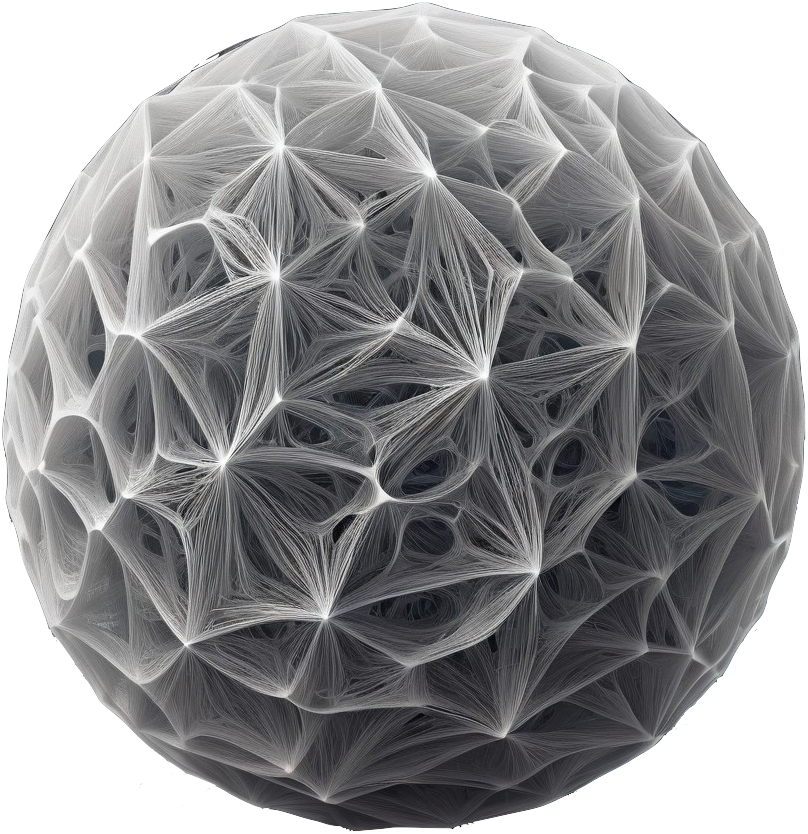
\includegraphics[width=.8\linewidth]{Figures/cover.png}
	\end{center}
	\vfill
	This course is taken in Spring 2024, and the date on the cover page is the last updated time.
\end{abstract}

\tableofcontents

\lec{1}{30}

\newpage
%─────Appendix────────────────────────────────────────────────────────────────────────────────────────────────────────────────────────────────────────
\appendix
\appendixpage{}

\chapter{Review}
\section{Boolean Satisfaction Problem}
Here, we give a quick review toward the \hyperref[prb:max-3SAT]{MAX-3SAT} problem.

\begin{definition}[Conjunctive normal form]\label{def:CNF}
	A \emph{conjunctive normal form} (CNF) formula is a conjunction \(\varphi\) of one or more boolean clauses on \(x_1, x_2, \dots  , x_n\) with boolean valued \(\{0, 1\}\). Explicitly, \(\varphi\) is in CNF if
	\[
		\varphi(x_1, x_2, \dots, x_n) = \text{clause}_1 \wedge \text{clause}_2 \wedge \text{clause}_3 \wedge \dots  \wedge \text{clause}_k
	\]
	where each clause is an or of literals, with a literal being some \(x_i\) or its negation \(\neg x_i\).
\end{definition}

\begin{note}[Disjunctive normal form]
	For every \hyperref[def:CNF]{conjunctive normal form}, there is an equivalent way to write it in the so-called \emph{disjunctive normal form}.
\end{note}

\begin{definition}[\(k\)-CNF]\label{def:k-CNF}
	A \emph{\(k\)-CNF formula} is a \hyperref[def:CNF]{CNF} formula in which each clause has exactly \(k\) literals from distinct variables.
\end{definition}

\begin{eg}[3-CNF]
	A \hyperref[def:k-CNF]{\(3\)-CNF formula} can be like
	\[
		\varphi = (x_1 \vee \neg x_2 \vee x_4) \wedge (\neg x_3 \vee x_4 \vee x_5) \wedge (\neg x_1 \vee \neg x_5 \vee \neg x_6).
	\]
\end{eg}

Now, the boolean satisfability problem asks the following question: given a \hyperref[def:k-CNF]{\(k\)-CNF formula} \(\varphi \), does an assignment exist such that \(\varphi \) is evaluated as true? Formally, we have \autoref{prb:k-SAT}.

\begin{problem}[\(k\)-SAT]\label{prb:k-SAT}
Given a \hyperref[def:k-CNF]{\(k\)-CNF formula} \(\varphi\), the \emph{\(k\)-SAT} problem asks whether \(\varphi\) is satisfiable.
\end{problem}

Instead of looking at a general \(k\), we consider a simple but also hard enough case when \(k = 3\). Specifically, we ask the following question.
\begin{problem}[MAX-3SAT]\label{prb:max-3SAT}
Given a \hyperref[def:k-CNF]{\(3\)-CNF formula} \(\varphi\) and \(\ell\), the \emph{MAX-3SAT} problem asks is there an assignment of variables such that it satisfies at least \(\ell \) clauses?
\end{problem}

\begin{remark}
	We often call \hyperref[prb:max-3SAT]{MAX-3SAT} as 3SAT for brevity.
\end{remark}

\subsection{Random MAX-3SAT}
A surprising result is that by randomly assigning \(x_i\), we achieve the best we can do in expectation. Algorithmically, we have the following.

\begin{algorithm}[H]\label{algo:random-max-3SAT}
	\DontPrintSemicolon{}
	\caption{Deterministic \hyperref[prb:max-3SAT]{MAX-3SAT}}
	\KwData{A \hyperref[def:k-CNF]{3-CNF} \(\varphi (x_1, \dots , x_n)\)}
	\KwResult{A \(7 / 8\)-approximation assignment \(\left\{ x_i \right\}_{i=1}^n\) (in expectation)}
	\SetKwFunction{unif}{uniform}
	\BlankLine

	\For(){\(i = 1, \dots  , n\)}{
		\(x_i\gets\)\unif{\(\left\{ 0, 1 \right\}\)}\Comment*[r]{random assignments}
	}
	\Return{\(\left\{ x_i \right\}_{i=1}^n\)}\;
\end{algorithm}

\begin{lemma}\label{lma:random-max-3SAT}
	For all \hyperref[def:k-CNF]{3-CNF} \(\varphi\), there exists an assignment that satisfies at least \(7 / 8\) of clauses.
\end{lemma}
\begin{proof}
	Each clause is satisfied by all but exactly \(1\) assignment, the one where all the literals in the clause evaluate to false. Imagine we have a uniformly random assignment of variables, and let \(X_i\) be a random variable such that
	\[
		X_i = \begin{dcases}
			1, & \text{ if \(i^{st} \) clause is satisfied}  ; \\
			0, & \text{ otherwise}.
		\end{dcases}
	\]

	Since each clause has \(8\) different possibilities (\(2^3\)), and there is only one situation where the clause is not satisfied, each clause has a probability of \(7 / 8\) of being satisfied. Therefore:
	\[
		\Pr(X_i = 1) = \frac{7}{8} = \mathbb{E}[X_i].
	\]
	Let \(X\) be a random variable that corresponds to the number of satisfied clauses, i.e., \(X = \sum_{i=1}^n X_i\).  By the linearity of expectation, we have
	\[
		\mathbb{E}[X] = \sum_{i=1}^n \mathbb{E}(X_i) = \frac{7}{8} \cdot m \geq \frac{7}{8}\OPT
	\]

	This shows that if we had an algorithm that randomly picks assignments of variables and checks to see how many clauses are satisfied, this would be a randomized algorithm that achieves \(\alpha = \frac{7}{8}\). If we were then to repeat the algorithm a polynomial number of times, we could show that there is a good chance to find such an assignment using Markov's inequality.
\end{proof}

\newpage
%─────Reference──────────────────────────────────────────────────────────────────────────────────────────────────────────────────────────────────────
\pagestyle{plain}
\printbibliography{}

\end{document}